\documentclass[../report.tex]{subfiles}
\graphicspath{{\subfix{../image/}}}

\begin{document}
\maketitle

\subsection{Lifting Development}
\begin{wrapfigure}{r}{0.5\textwidth}
    \centering
    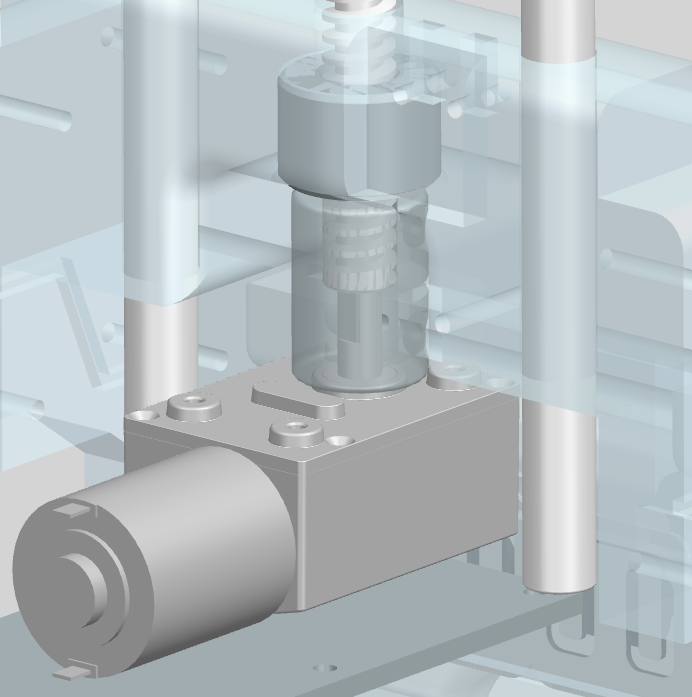
\includegraphics[width=0.5\textwidth]{mast2.png}
    \caption{JGY370 with lead screw}
\end{wrapfigure}
Through choosing the lead screw as a lifting solutions we have to find the
the minimum torque our motor has to put out in order drive the screw under full load.
As we got our lifting motor, the JGY370 sourced in the beginning of the semester without 
any of the further calculations, this will also state if it will fit our project requirements.

To find the Torque, which our Motor has to supply we derive from $Torque=Force*Distance$, where the 
distance is the radius of the lead screw and the force is the force of the load divided by the Mechanical 
Advantage gained through the lead screw. $F_{total}=F_{Load}/MA$

\[F_{Load}=Mass*G=3.5kg*9.81\frac{m}{s}=34.34N\]

The Mechanical Advantage is the product of Velocity Ratio and Efficiency dependent on the lead 
angle. $MA=VR*E$ 

\[VR=\frac{Circumference}{Lead}=\frac{(\pi*10)}{1}=15.7\]

Efficiency shows the impact of friction on the system, which can be accounted for as as increase in lead angle of the threads 
as in the ratio between angle and friction angle. A higher friction results therefore equally to adding more load in an ideal 
system. The friction in this case is described as the \cite{friction_coefficient}[static 
friction coefficient of hard steel on hard steel] as it is the highest to overcome. 

\[friction.angle=atand(friction.coefficient)= atand(0.42)=22.8\]
\[E=\frac{tand(lead.angle)}{tand(lead.angle+friction.angle)}=\frac{tand(3.64)}{tand(3.64+22.8)}=0.13\]

From where we now have all to calculate the needed torque, 
\[F_{total}=\frac{34.4N}{15.7*0.13}=17N\]
\[Torque=17N*0.005m=0.085Nm\quad or \quad 8.5Ncm\]

The JGY370 is rated at 235 Ncm and so sufficient for our use case. With it´s 50 RPM
lifting 15cm are very slow, as one way would take 90 seconds. For the goal off lifting 
our load 15cm in 10 seconds we would have needed a motor with 450 rpm, which was not 
available for the JGY370.

Because redesigning and finding at new motor 
or completely changing the lifting solution was not an option as the mechanical design 
was not the priority in this semester project, we decided to keep the working but slow 
solution as a proof of concept. This allowed us to focus on the electronics and sensor 
implementation and staying within our timeline.


\end{document}